\documentclass[
  % all of the below options are optional and can be left out
  % course name (default: 2IL50 Data Structures)
  course = {{ESE532 System-on-a-Chip}},
  % quartile (default: 3)
  quartile = {{}},
  % assignment number/name (default: 1)
  assignment = 2,
  % student name (default: Some One)
  name = {{Sheil Sarda}},
  % student number, NOT S-number (default: 0123456)
  studentnumber = {{}},
  % student email (default: s.one@student.tue.nl)
  email = {{sheils@seas.upenn.edu}},
  % first exercise number (default: 1)
  firstexercise = 1
]{aga-homework}
\usepackage{graphicx} 

\begin{document}

\exercise
\subexercise Scale: down-samples the input array by a factor of two, transforming an image of size $HEIGHT * WIDTH$ to an image of size $(HEIGHT / 2) * (WIDTH / 2)$. The index used inside the nested for-loop ($Y * WIDTH + X$) is used to access the pixel located at $(X, Y)$, assuming the origin of the coordinate system is located in the top-left corner.
\begin{verbatim}
void Scale(const unsigned char * Input, unsigned char * Output){
  for (int Y = 0; Y < HEIGHT; Y += 2)
    for (int X = 0; X < WIDTH; X += 2)
      Output[(Y / 2) * WIDTH / 2 + (X / 2)] = Input[Y * WIDTH + X];
}
\end{verbatim}


\subexercise Filter:
\begin{itemize}
  \item \verb Filter  applies a horizontal and vertical filter to the input image, and returns the filtered image as the output.
  \item \verb Filter_horizontal  scans through every pixel of the image, and replaces it with \verb SUM  divided by 256. \verb SUM  is the value of each Coefficient, where coefficients add up to 256, multiplied by the value stored in each pixel. In effect, this smooths each pixel of the image by replacing the value with a weighted average of the pixels in the same row, or for pixels on the edge-- a weighted average of pixels in the adjacent row. 
  \item \verb Filter_vertical  functions the same way as \verb Filter_horizontal  except that it replaces each pixel with a weighted average of the pixels in the same column, or for pixels on the edge-- a weighted average of pixels in adjacent columns.
\end{itemize} 

\begin{verbatim}
void Filter(const unsigned char * Input, unsigned char * Output){
  unsigned char * Temp = (unsigned char*)malloc(INPUT_HEIGHT * OUTPUT_WIDTH);
  Filter_horizontal(Input, Temp);
  Filter_vertical(Temp, Output);
  free(Temp);
}

void Filter_horizontal(const unsigned char * Input, unsigned char * Output){
  for (int Y = 0; Y < INPUT_HEIGHT; Y++)
    for (int X = 0; X < OUTPUT_WIDTH; X++){
      unsigned int Sum = 0;
      for (int i = 0; i < FILTER_LENGTH; i++)
        Sum += Coefficients[i] * Input[Y * INPUT_WIDTH + X + i];
      Output[Y * OUTPUT_WIDTH + X] = Sum >> 8;
    }
}

static void Filter_vertical(const unsigned char * Input, unsigned char * Output){
  for (int Y = 0; Y < OUTPUT_HEIGHT; Y++)
    for (int X = 0; X < OUTPUT_WIDTH; X++){
      unsigned int Sum = 0;
      for (int i = 0; i < FILTER_LENGTH; i++)
        Sum += Coefficients[i] * Input[(Y + i) * OUTPUT_WIDTH + X];
      Output[Y * OUTPUT_WIDTH + X] = Sum >> 8;
    }
}
\end{verbatim}

\subexercise Differentiate: Replaces each pixel of the image with the difference of the input and \verb AVERAGE . \verb AVERAGE  is defined as the arithmetic mean of the value of the pixels located directly above and to the left of the current pixel. For edge cases where the previous row or column may not exist, we simply use either previous row or previous column.
\begin{verbatim}
void Differentiate(const unsigned char * Input, unsigned char * Output){
  for (int Y = 0; Y < HEIGHT; Y++)
    for (int X = 0; X < WIDTH; X++){
      int Average = 0;
      if (Y > 0 && X > 0)
        Average = (Input[WIDTH * (Y - 1) + X] + Input[WIDTH * Y + X - 1]) / 2;
      else if (Y > 0)
        Average = Input[WIDTH * (Y - 1) + X];
      else if (X > 0)
        Average = Input[WIDTH * Y + X - 1];
      unsigned char Diff = Input[WIDTH * Y + X] - Average;
      Output[Y * WIDTH + X] = Diff;
    }
}
\end{verbatim}

\subexercise Compress: for each pixel in the image, first fetch the corresponding \verb Code and  \verb Code_length  using the pixel value. Then, computer \verb Byte by bit-shifting the current value to the right, and filling it in with the bit-sequence in \verb Code , but reverse order. When Byte reaches a length of 8 digits, it gets put into the \verb Output  array, and the local variable is reset to 0 to start again. The \verb Output  array is thus $\frac{1}{8}$ the size of the \verb Input  array, and each value in the array is a \verb Code .
\begin{verbatim}
int Compress(const unsigned char * Input, unsigned char * Output){
  unsigned int Byte = 0;
  int Length = 0;
  for (int i = 0; i < SIZE; i++){
    unsigned long long Code = Codes[Input[i]];
    int Code_length = Code_lengths[Input[i]];

    for (int j = 0; j < Code_length; j++){
      Byte = (Byte << 1) | ((Code >> (Code_length - 1 - j)) & 1);

      if (++Length % 8 == 0){
        Output[Length / 8 - 1] = Byte;
        Byte = 0;
      }
    }
  }
  if (Length % 8 > 0)
    Output[Length / 8] = Byte;
  return Length / 8 + 1;
}
\end{verbatim}



\exercise

\subexercise 
\begin{center}
  \begin{tabular}{||c | c | c | c | c||} 
    \hline
    Functions & Average Latency       & \% of total latency & Average Latency (2.3 GHz)    & Actual Latency     \\ [0.5ex] 
           & ($T_{measured\_avg}$ ns) & (1.28811e+08 ns)     & ($T_{measured\_avg}$ cycles) & (\% of total cycles)  \\ [0.5ex] 
    \hline\hline
    Scale         & 3.93261e+06  & 3.05\% & 9,045,003  & 9,237,036 \\ 
    \hline
    Filter horizontal   & 2.94201e+07  & 22.84\% & 67,666,230  & 69,171,771 \\
    \hline
    Filter vertical   & 3.26903e+07  & 25.38\% & 75,187,690  & 76,864,253 \\
    \hline
    Differentiate     & 8.56184e+06  & 6.65\% & 19,692,232  & 20,139,767  \\
    \hline
    Compress       & 4.59722e+07  & 35.69\% & 105,736,060  & 108,087,414    \\ [1ex] 
    \hline
  \end{tabular}
\end{center}

\exercise

\subexercise
  From the above table, the function with the highest latency alone is compress. 
  \newline
  \newline 
  If we include filter in this comparison, which is comprised of filter horizontal and vertical, it would have the highest latency.
\subexercise
  DFG of the body of the loop over $x$:
  \newpage
  \begin{figure}
    \centering
    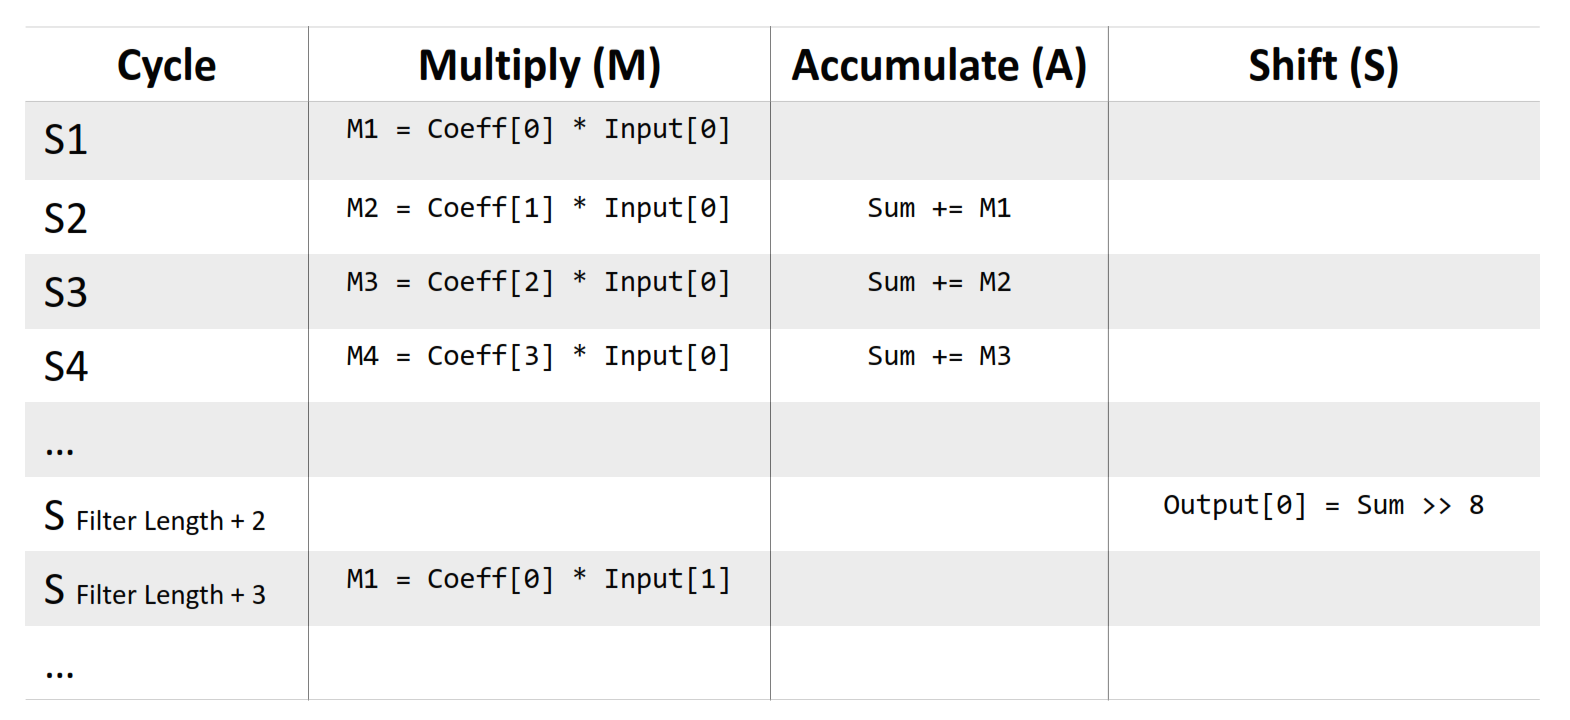
\includegraphics[width=0.7\linewidth]{figures/dfg_1}
    \caption{Instructions executed each cycle, excluding memory accesses for INPUT and Coefficients array, since those instructions were not mentioned in the submission guidelines.}
    \label{fig:usagereport}
  \end{figure}
  \begin{figure}
    \centering
    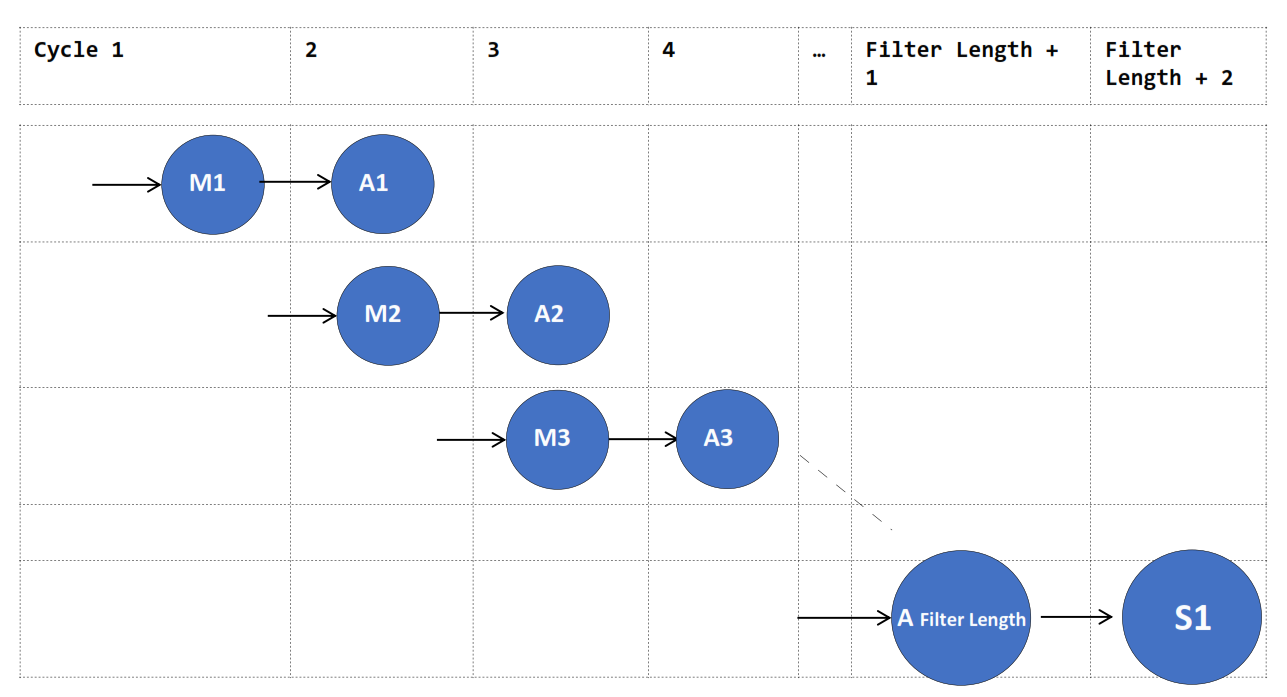
\includegraphics[width=0.7\linewidth]{figures/dfg_2}
    \caption{Data Flow Graph with timing information}
    \label{fig:usagereport}
  \end{figure}
  
\begin{verbatim}
void Filter_horizontal(const unsigned char * Input, unsigned char * Output)  {
  for (int Y = 0; Y < INPUT_HEIGHT*OUTPUT_WIDTH; Y++) {
    unsigned int Sum = 0;
    for (int i = 0; i < FILTER_LENGTH; i++)  
      Sum += Coefficients[i] * Input[Y + i];

    Output[Y] = Sum >> 8;
  }
}  
\end{verbatim}
\subexercise
Total number of compute operations equals $(\verb FILTER_LENGTH * 3 + 2)*(1500*2000) = 69,000,000$. This number excludes loop overhead, and assumes that memory fetches from the \verb INPUT  and \verb Coefficients  array can occur in one cycle each.

\subexercise The $2 \times$ speed-up should be applied to the slowest segment of the code, which as we discussed above, is the compress function. This function currently comprises $\sim 36\%$ of the total latency.

\subexercise Assuming we speedup the compress function by a factor of $2 \times$, $T_{after} = \frac{1}{2}*35.69\% + 1*(1-35.69\%) = 0.82$. The resulting speedup = $\frac{T_{before}}{T_{after}} = \frac{1}{0.82} = 1.22\times$.
\newpage
\subexercise New Data Flow Graph with lowest critical path delay.
  \begin{figure}
	\centering
	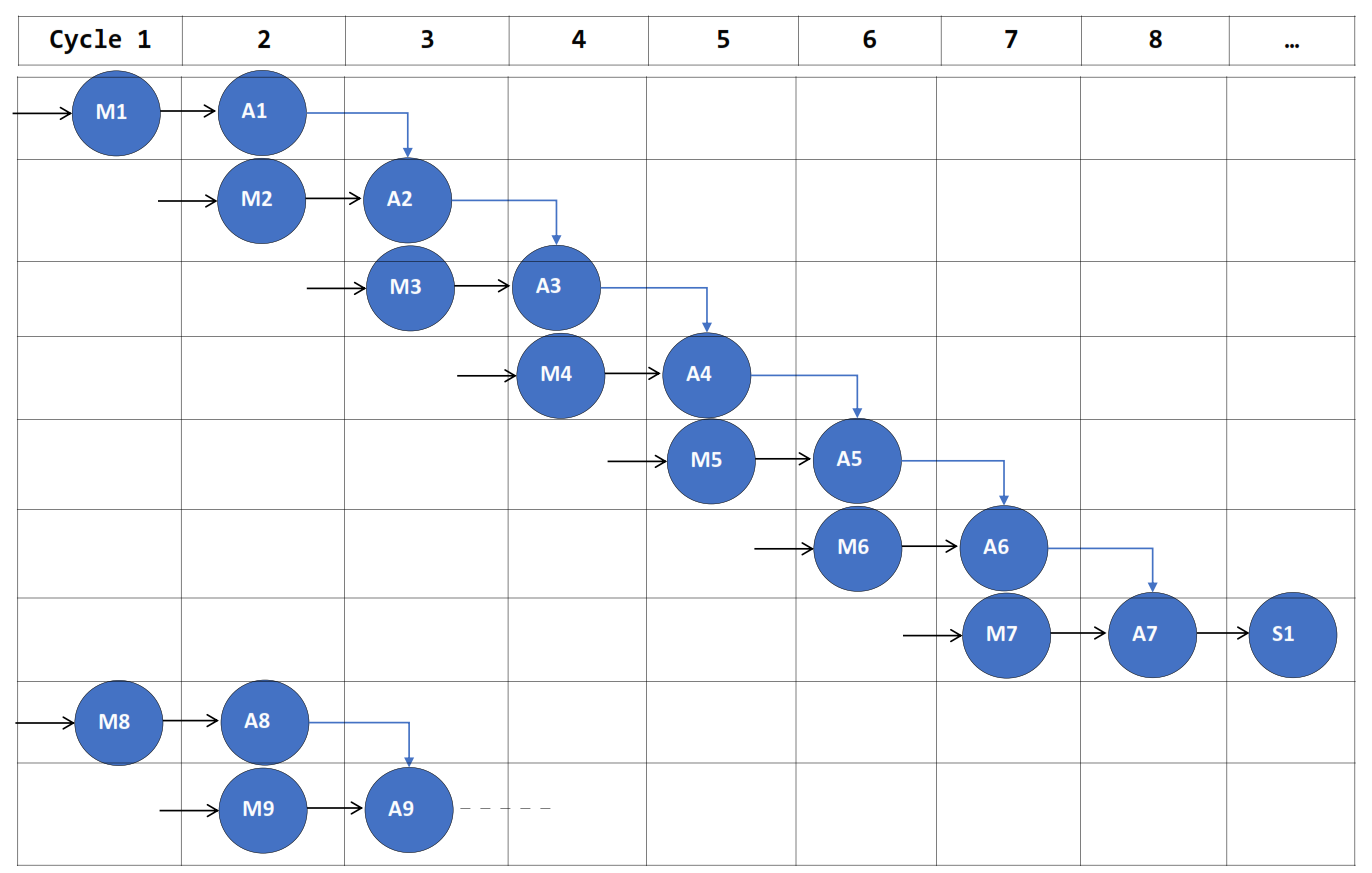
\includegraphics[width=0.7\linewidth]{figures/dfg_3}
	\caption{Data Flow Graph assuming unlimited resources.}
	\label{fig:usagereport}
\end{figure}
\subexercise New critical path length assuming instructions can execute in the same cycle in terms of compute operations is \verb FILTER_LENGTH  + 2 cycles assuming addition, multiplication and bit-shift operations take a single cycle to execute. 

\subexercise Resource capacity lower bound for the loop body assuming 4 multipliers, 2 adders and 1 shifter is $\frac{Total Ops}{Operators}$
\begin{itemize}
	\item Total \# of add operations: $7 * (1500*2000) = 21,000,000$. Since we have 2 adders, $RB_{ADD} = 10,500,000$.
	\item Total \# of multiplication operations is $21,000,000$ using the same logic. Since we have 4 multipliers, $RB_{MULT} = 5,250,000$.
	\item Total \# of shift operations is $3,000,000$. Since we have 1 shifter, $RB_{SHIFT} = 3,000,000$.
\end{itemize}
The overall Resource Bound of the algorithm is the max of the above bounds. In this case, $RB = 10,500,000$ cycles.
\newline \newline
For a single loop iteration, 
\begin{itemize}
	\item $RB_{ADD} = 3.5$.
	\item $RB_{MULT} = 1.75$.
	\item $RB_{SHIFT} = 1$.
\end{itemize}
The $RB$ would equal $3.5$ cycles, bottle-necked by the adders.
\newpage
\exercise
\subexercise
\begin{verbatim}
(gdb) n
  60              Sum += Coefficients[i] * Input[Y * INPUT_WIDTH + X + i];
(gdb) disassemble
  Dump of assembler code for function Filter_horizontal:
  0x00000000004014a0 <+0>:     add     x9, x0, \#0x2dc, lsl \#12
  0x00000000004014a4 <+4>:     adrp    x6, 0x420000
  0x00000000004014a8 <+8>:     add     x8, x0, \#0x7ca
  0x00000000004014ac <+12>:    add     x9, x9, \#0xe8a
  => 0x00000000004014b0 <+16>:    add     x6, x6, \#0xcc0
  0x00000000004014b4 <+20>:    sub     x5, x8, \#0x7ca
  0x00000000004014b8 <+24>:    mov     x7, x1
  0x00000000004014bc <+28>:    nop
  0x00000000004014c0 <+32>:    mov     x0, \#0x0                        // \#0
  0x00000000004014c4 <+36>:    mov     w2, \#0x0                        // \#0
  0x00000000004014c8 <+40>:    ldrb    w4, [x5, x0]
  0x00000000004014cc <+44>:    ldr     w3, [x6, x0, lsl \#2]
  0x00000000004014d0 <+48>:    add     x0, x0, \#0x1
  0x00000000004014d4 <+52>:    cmp     x0, \#0x7
  0x00000000004014d8 <+56>:    madd    w2, w4, w3, w2
  0x00000000004014dc <+60>:    b.ne    0x4014c8 <Filter_horizontal+40>  // b.any
  0x00000000004014e0 <+64>:    lsr     w2, w2, \#8
  0x00000000004014e4 <+68>:    strb    w2, [x7], \#1
  0x00000000004014e8 <+72>:    add     x5, x5, \#0x1
  0x00000000004014ec <+76>:    cmp     x8, x5
  0x00000000004014f0 <+80>:    b.ne    0x4014c0 <Filter_horizontal+32>  // b.any
  0x00000000004014f4 <+84>:    add     x8, x8, \#0x7d0
  0x00000000004014f8 <+88>:    add     x1, x1, \#0x7ca
  0x00000000004014fc <+92>:    cmp     x9, x8
  0x0000000000401500 <+96>:    b.ne    0x4014b4 <Filter_horizontal+20>  // b.any
  0x0000000000401504 <+100>:   ret
  End of assembler dump.
\end{verbatim}
\subexercise
\begin{center}
  \begin{tabular}{|| >{\ttfamily\catcode`_=12 }l | c | c | c | c | c ||} 
    \hline
    Assembly   & Annotation  & $\#$ of function   & $\#$ of cycles & $\#$ of instructions & Total cycles  \\ [0.5ex] 
    Instructions&         & calls ($N$)    & per call ($T$) & issued ($N_{issue}$)    & ($T \times N$)\\ [0.5ex] 
    \hline\hline
    add     x6, x6, \#0xcc0      & loop incr   &    1500  &1    &3    & 500  \\ 
    sub     x5, x8, \#0x7ca      &  fetch var    &  1500    &1  &3    &  500  \\ 
    mov     x7, x1      & fetch var     &  2000   &1   &3    & 667  \\ 
    mov     x0, \#0x0      & reset sum     &   3,000,000   &1    &3    & 1,000,000  \\ 
    mov     x0, \#0x0       &   reset sum   &  3,000,000    &1   &3    & 1,000,000   \\ 
    ldrb    w4, [x5, x0]      &   array read   & 21,000,000     &1  &3    & 7,000,000  \\ 
    ldr     w3, [x6, x0, lsl \#2]      &  array read    & 21,000,000      &1  &3    & 7,000,000  \\ 
    add     x0, x0, \#0x1      & index add     & 21,000,000      &1    &3   & 7,000,000  \\ 
    cmp     x0, \#0x7      & loop limit     &  21,000,000    &1    &3    & 7,000,000  \\ 
    madd    w2, w4, w3, w2      &  coeff mult     &  21,000,000    &1   &3    & 7,000,000  \\ 
    b.ne    0x4014c8      &  branch    &  21,000,000     &1  &3    &7,000,000   \\ 
    lsr     w2, w2, \#8     & div by 256      & 3,000,000    &1  &3    & 1,000,000  \\ 
    strb    w2, [x7], \#1      & store out  &   3,000,000  &1  &3  & 1,000,000  \\ 
    add     x5, x5, \#0x1      &  index add    &  3,000,000   &1  &3    & 1,000,000  \\ 
    cmp     x8, x5      & loop limit      &  3,000,000   &1    &3  &  1,000,000 \\ 
    b.ne    0x4014c0      &  branch    &  3,000,000   &1   &3   & 1,000,000  \\ 
    add     x8, x8, \#0x7d0     &  add to sum    &  1500     &1  &3    &  500 \\ 
    add     x1, x1, \#0x7ca     &  add to sum     & 1500     &1    &3    &  500 \\ 
    cmp     x9, x8     & loop limit      & 1500     &1  &3   &500   \\ 
    b.ne    0x4014b4      &   branch   &  1500   &1   &3   & 500  \\ 
   ret     &  return    & 1     &1   &3   &0   \\    
       \hline\hline       
    &     &     &   &   & 49,003,667   \\                       
    \hline
	\end{tabular}
\end{center}

\subexercise Other instructions in the above table are used to:
\begin{itemize}
	\item Divide Sum by 256 before array store. This is performed through bit-shifting operations.
	\item Store new pixel value to the Output array.
	\item Fetch variables to a register for loop limit comparisons.
	\item Reset Sum to 0 at the beginning of the iteration.
	\item Return statement at the end of the function.
\end{itemize} 
\subexercise Completed in table.

\subexercise Compute latency of non-memory instructions.
\begin{center}
	\begin{tabular}{|| >{\ttfamily\catcode`_=12 }l | c | c | c | c | c ||} 
		\hline
		Assembly   & Annotation  & $\#$ of function   & $\#$ of cycles & $\#$ of instructions & Total cycles  \\ [0.5ex] 
		Instructions&         & calls ($N$)    & per call ($T$) & issued ($N_{issue}$)    & ($T \times N$)\\ [0.5ex] 
		\hline\hline
		add     x6, x6, \#0xcc0      & loop incr   &    1500  &1    &3    & 500  \\ 
		sub     x5, x8, \#0x7ca      &  fetch var    &  1500    &1  &3    &  500  \\ 
		mov     x7, x1      & fetch var     &  2000   &1   &3    & 667  \\ 
		mov     x0, \#0x0      & reset sum     &   3,000,000   &1    &3    & 1,000,000  \\ 
		mov     x0, \#0x0       &   reset sum   &  3,000,000    &1   &3    & 1,000,000   \\ 
		add     x0, x0, \#0x1      & index add     & 21,000,000      &1    &3   & 7,000,000  \\ 
		cmp     x0, \#0x7      & loop limit     &  21,000,000    &1    &3    & 7,000,000  \\ 
		madd    w2, w4, w3, w2      &  coeff mult     &  21,000,000    &1   &3    & 7,000,000  \\ 
		b.ne    0x4014c8      &  branch    &  21,000,000     &1  &3    &7,000,000   \\ 
	    lsr     w2, w2, \#8     & div by 256      & 3,000,000    &1  &3    & 1,000,000  \\ 
		add     x5, x5, \#0x1      &  index add    &  3,000,000   &1  &3    & 1,000,000  \\ 
		cmp     x8, x5      & loop limit      &  3,000,000   &1    &3  &  1,000,000 \\ 
		b.ne    0x4014c0      &  branch    &  3,000,000   &1   &3   & 1,000,000  \\ 
		add     x8, x8, \#0x7d0     &  add to sum    &  1500     &1  &3    &  500 \\ 
		add     x1, x1, \#0x7ca     &  add to sum     & 1500     &1    &3    &  500 \\ 
		cmp     x9, x8     & loop limit      & 1500     &1  &3   &500   \\ 
		b.ne    0x4014b4      &   branch   &  1500   &1   &3   & 500  \\ 
		ret     &  return    & 1     &1   &3   &0   \\    
		\hline\hline       
		&     &     &   &   & 34,003,667   \\                       
		\hline
	\end{tabular}
\end{center}

$$T_{cycle\_memory} = T_{total} - T_{non\_memory}  = 67,666,230 - 34,003,667 = 33,662,563$$

\subexercise 
Identified memory operations, and if the ops are to memory locations not loaded during invocation of the function.
\begin{center}
	\begin{tabular}{|| >{\ttfamily\catcode`_=12 }l | c | c | l | c ||} 
		\hline
		Assembly   & Annotation  & $\#$ of function & Previously  & \% of total\\ [0.5ex] 
		Instructions&         & calls ($N$)  & observed (Y/N) & cycles \\ [0.5ex] 
		\hline\hline
		ldrb    w4, [x5, x0]      &   array read   & 21,000,000 & Y (coeff.) & 14.29\% \\ 
		ldr     w3, [x6, x0, lsl \#2]      &  array read    & 21,000,000 & N (Input) & 14.29\% \\ 
		strb    w2, [x7], \#1      & output  &   3,000,000 & N (Output) & 2.04\% \\     
		\hline
	\end{tabular}
\end{center}
Estimates for different quantities in the timing equation:
$$N_{total} = 147,011,001 \text{ cycles}$$
$$N_{slow\_loads} = 24,000,000 \text{ cycles}$$
$$N_{fast\_loads} = 21,000,000 \text{ cycles}$$
\subexercise

We know:
$$T_{cycle\_memory} = 33,662,563  = T_{fast\_loads} + T_{slow\_loads} $$
Also:
$$T_{fast\_loads} = \frac{21,000,000}{3} \times 1 = 7,000,000 $$
Substituting in the original equation, we get:
$$T_{slow\_loads} = 33,662,563 - 7,000,000 = 26,662,563 \text{ cycles} $$
\end{document}
